\usetikzlibrary{arrows.meta,calc,decorations.pathreplacing}
\usetikzlibrary{circuits.logic.US}

\tikzset{
    simple wire/.style={very thick,>=Latex},
    wire/.style={line width=1.5pt,>=Latex},
    wire thick/.style={line width=2.5pt,>=Latex},
    wire small/.style={line width=1pt,>=Latex},
    binLabel/.style={font=\tt},
    hiBox/.style={red, very thick, draw}
}

\begin{frame}{HCLRS: wire (bundle)s}
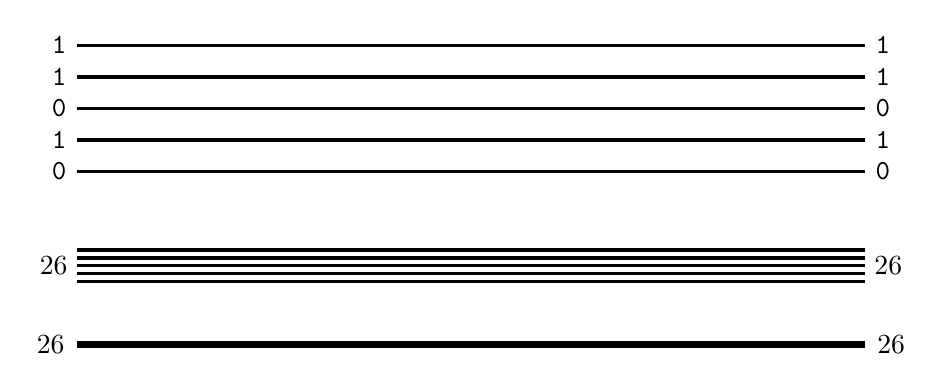
\begin{tikzpicture}
\foreach \x/\v in {0/0,0.4/1,0.8/0,1.2/1,1.6/1} {
    \draw[simple wire] (0, \x) node[left,binLabel] (\x-\v-num) {\v} -- (10, \x) node[right,binLabel]{\v};
};
\begin{scope}[yshift=-1.4cm]
\foreach \x in {0,0.1,0.2,0.3,0.4} {
    \draw[simple wire] ($(0, \x) + (0, 0)$) -- ($(10, \x) + (0, 0)$);
};
\node[anchor=east] at (0, 0.2) {26};
\node[anchor=west] at (10, 0.2) {26};
\end{scope}
\begin{scope}[yshift=-2.2cm]
\draw[wire thick] (0, 0) node[left] {26} -- ++(10, 0) node[right] {26};
\end{scope}
\end{tikzpicture}
\begin{itemize}
\item \texttt{wire \tikzmark{startName1a}foo\tikzmark{endName1a} : \tikzmark{startWidth1a}5\tikzmark{endWidth2a}; \tikzmark{startAssign1a}foo = 0b11010\tikzmark{endAssign1a};} \hspace{0.7cm} \textit{OR}
\item \texttt{wire \tikzmark{startName2a}foo\tikzmark{endName2a} : \tikzmark{startWidth2a}5\tikzmark{endWidth2a}; foo = 26;} \hspace{2.25cm} \textit{OR}
\item \texttt{wire \tikzmark{startName3a}foo\tikzmark{endName3a} : \tikzmark{startWidth3a}5\tikzmark{endWidth3a}; \tikzmark{startAssign3a}foo = 0x1a\tikzmark{endAssign3a};}
\end{itemize}
\begin{tikzpicture}[overlay,remember picture]
\begin{visibleenv}<2>
\coordinate (nameTopLeftA) at ([yshift=1em]pic cs:startName1a);
\coordinate (nameBottomRightA) at ([yshift=-.25em]pic cs:endName3a);
\coordinate (nameBottomLeftA) at (nameBottomRightA -| nameTopLeftA);
\coordinate (nameBottomCenterA) at ($(nameBottomRightA)!0.5!(nameBottomLeftA)$);
\draw[red,very thick] (nameTopLeftA) rectangle (nameBottomRightA);
\node[anchor=north] at (nameBottomCenterA) {
    \textit{name}
};
\end{visibleenv}
\begin{visibleenv}<3>
\coordinate (widthTopLeftA) at ([yshift=1em]pic cs:startWidth1a);
\coordinate (widthBottomRightA) at ([yshift=-.25em]pic cs:endWidth3a);
\coordinate (widthBottomLeftA) at (widthBottomRightA -| widthTopLeftA);
\coordinate (widthBottomCenterA) at ($(widthBottomRightA)!0.5!(widthBottomLeftA)$);
\draw[red,very thick] (widthTopLeftA) rectangle (widthBottomRightA);
\node[anchor=north] at (widthBottomCenterA) {
    \textit{width} (in bits)
};
\end{visibleenv}
\begin{visibleenv}<4>
\coordinate (assignTopLeftA) at ([yshift=1em]pic cs:startAssign1a);
\coordinate (assignBottomRightA) at ([yshift=-.25em,xshift=1.75cm]pic cs:endAssign3a);
\coordinate (assignBottomLeftA) at (assignBottomRightA -| assignTopLeftA);
\coordinate (assignBottomCenterA) at ($(assignBottomRightA)!0.5!(assignBottomLeftA)$);
\draw[red,very thick] (assignTopLeftA) rectangle (assignBottomRightA);
\node[anchor=north,align=center] at (assignBottomCenterA) {
    \textit{assignment} \\
    indicates wire is \textit{connected} to value
};
\end{visibleenv}
\end{tikzpicture}
\end{frame}

\begin{frame}{HCLRS: gates + calcuations (1)}
\texttt{wire a : 2; wire b : 2; wire c : 2;} \\
\texttt{c = \myemph<3>{b \& a};}\tikzmark{afterCAssign} \\
\texttt{a = 0b10;} \\
\texttt{b = 0b11;}
\vspace{2cm}
\begin{tikzpicture}[overlay,remember picture]
\begin{visibleenv}<2>
\node[align=left,font=\tt,anchor=north west] (alt code) at ([yshift=1em,xshift=3cm]pic cs:afterCAssign) {
a = 0b10; \\
b = 0b11; \\
c = \myemph<3>{b \& a};
};
\node[red] at ([xshift=-1.5cm]alt code.west) {same as};
\draw[red,decorate,decoration={brace},ultra thick] ([xshift=-2.9cm]alt code.north west) -- ([xshift=-2.9cm]alt code.south west);
\draw[red,decorate,decoration={brace,mirror},ultra thick] ([xshift=-0.1cm]alt code.north west) -- ([xshift=-0.1cm]alt code.south west);
\node[anchor=north,red,align=center] at ([xshift=-1.5cm,yshift=-.25cm]alt code.south west) {
    \textbf{order doesn't matter} \\
    connected or not
};
\end{visibleenv}
\begin{visibleenv}<3>
\node[anchor=north,red,align=center] at ([xshift=2cm,yshift=.9cm]alt code.west) {
    C-like expressions supported \\
    \texttt{0b10 \& 0b11 = 0b10}
};
\end{visibleenv}
\end{tikzpicture}

\begin{tikzpicture}[circuit logic US]
\draw[wire] (0, -.05) -- ++(3, 0) coordinate (end A bot);
\draw[wire] (0, .05) -- ++(3, 0) node[midway,yshift=-.05cm,fill=white,font=\tt] {a} coordinate (end A top);
\draw[wire] (0, -1.05) -- ++(3, 0) coordinate (end B bot);
\draw[wire] (0, -0.95) -- ++(3, 0) node[midway,yshift=-.05cm,fill=white,font=\tt] {b} coordinate (end B top);
\node[alt=<3>{red},thick,and gate,label={[alt=<3>{red},font=\scriptsize]center:AND},anchor=input 1] (and-1) at (5, .05) {};
\draw[wire] (end A top) -- (and-1.input 1);
\draw[wire] (end B top) -- ++ (0.75, 0) |- (and-1.input 2);
\node[alt=<3>{red},thick,and gate,label={[alt=<3>{red},font=\scriptsize]center:AND},anchor=input 2] (and-2) at (5, -1.05) {};
\draw[white,line width=3pt] (end A bot) -- ++(1.5, 0) |- (and-2.input 1);
\draw[wire] (end A bot) -- ++ (1.5, 0) |- (and-2.input 1);
\draw[wire] (end B bot) -- (and-2.input 2);

\coordinate (c height) at ($(and-1.output)!0.5!(and-2.output)$);
\coordinate (c join) at ([xshift=2cm]c height);
\draw[wire] (and-1.output) -- ++(1, 0) |- ([yshift=.05cm]c join) -- ++(2, 0);
\draw[wire] (and-2.output) -- ++(1, 0) |- ([yshift=-.05cm]c join) -- ++(2, 0);
\node[fill=white] at ([xshift=1cm]c join) {c};
\end{tikzpicture}
\end{frame}

\begin{frame}{HCLRS: gates + calcuations (2)}
\texttt{wire a : 2; wire b : 2; wire c : 2;} \\
\texttt{\myemph<1>{c = \large b \textbf{+} a}; /* was \sout{b \& a} */}\tikzmark{afterCAssign} \\
\texttt{a = 0b10;} \\
\texttt{b = 0b11;}
\vspace{2cm}
\begin{tikzpicture}[overlay,remember picture]
\begin{visibleenv}<1>
\node[anchor=north,red,align=center] at ([xshift=2cm,yshift=-0.5cm]alt code.west) {
    more than bitwise operators supported \\
    0b10 + 0b11 = 0b101 $\rightarrow$ 0b01 (extra bits lost)
};
\end{visibleenv}
\end{tikzpicture}

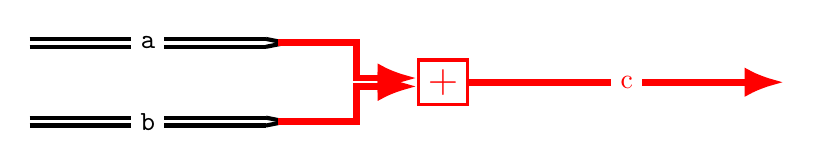
\begin{tikzpicture}[circuit logic US]
\draw[wire] (0, -.05) -- ++(3, 0) coordinate (end A bot);
\draw[wire] (0, .05) -- ++(3, 0) node[midway,yshift=-.05cm,fill=white,font=\tt] {a} coordinate (end A top);
\coordinate (end A mid inter) at ($(end A bot)!0.5!(end A top)$);
\coordinate (end A mid) at ([xshift=.25cm]end A mid inter);
\draw[wire] (end A bot) -- (end A mid);
\draw[wire] (end A top) -- (end A mid);
\draw[wire] (0, -1.05) -- ++(3, 0) coordinate (end B bot);
\draw[wire] (0, -0.95) -- ++(3, 0) node[midway,yshift=-.05cm,fill=white,font=\tt] {b} coordinate (end B top);
\coordinate (end B mid inter) at ($(end B bot)!0.5!(end B top)$);
\coordinate (end B mid) at ([xshift=.25cm]end B mid inter);
\draw[wire] (end B bot) -- (end B mid);
\draw[wire] (end B top) -- (end B mid);

\coordinate (end mid) at ($(end A mid)!0.5!(end B mid)$);

\node[red,draw,very thick,font=\Large] (add box) at ([xshift=2cm]end mid) {+};
\draw[red,wire thick,-Latex] ([xshift=-1mm]end A mid) -- ++ (1, 0) |- ([yshift=-.25cm]add box.north west);
\draw[red,wire thick,-Latex] ([xshift=-1mm]end B mid) -- ++ (1, 0) |- ([yshift=+.25cm]add box.south west);
\draw[red,wire thick,-Latex] (add box.east) -- ++ (4, 0) node[midway,fill=white] {c};
\end{tikzpicture}
\end{frame}
